%\documentclass{beamer}
\documentclass[handout]{beamer}

\usepackage[brazilian]{babel}
\usepackage[utf8]{inputenc}
\usepackage{graphicx}
\usepackage{fontenc}
\usepackage{listings}
\usepackage{verbatim}
\usepackage{pxfonts}
\usepackage{graphicx}
\usetheme{Amsterdam}

\title{Grandes Migrações com o WordPress}
\subtitle{Passando de qualquer plataforma \\
  para o WordPress}
\author{Vinicius Massuchetto}
\date{}

\lstset{%
  breakatwhitespace,
  columns=fullflexible,
  keepspaces,
  breaklines,
  tabsize=2,
  showstringspaces=false,
  extendedchars=true,
  basicstyle=\footnotesize\ttfamily,
  frame=leftline}

\begin{document}

\frame{\titlepage}

\section{Introdução}
\subsection{Introdução}

\begin{frame}{Download}
  \begin{center}

    Código fonte da apresentação:

    \vspace{0.1cm}

    \url{https://github.com/vmassuchetto/wp-migrations}

    \vspace{0.1cm}

    \footnotesize{(branch intercon)}

    \vspace{1cm}

    PDF compilado:

    \vspace{0.1cm}

    \url{http://tinyurl.com/intercon-migracoes}

  \end{center}
\end{frame}

\begin{frame}{Sobre o que falaremos}
  \tableofcontents[subsectionstyle=hide]
\end{frame}

\section{Motivação}
\subsection{Motivação}

\begin{frame}{Por que falar sobre migrações com o cliente?}
\begin{itemize}
  \pause \item Indexação de conteúdo
  \pause \item Manutenção de usabilidade
  \pause \item Reestruturação do conteúdo
\end{itemize}
\end{frame}

\begin{frame}{Por que falar sobre migrações com a equipe de desenvolvimento?}
\begin{itemize}
  \pause \item Análise de complexidade
  \pause \item Análise de correlação e criação de estruturas
  \pause \item Resolução de velhos problemas
  \pause \item Definição de estratégias
  \pause \item Delegação de tarefas
  \pause \item Elaboração de manuais
  \pause \item Definição do tempo de projeto
\end{itemize}
\end{frame}

\begin{frame}{E na verdade, as migrações são..}
\begin{itemize}
  \pause \item Uma etapa de projeto que poderia ser melhor discutida
  \pause \item Uma das partes mais importantes da implantação de projetos web
\end{itemize}
\end{frame}

\section{Migrações Simples}
\subsection{Migrações Simples}

\begin{frame}
\frametitle{O que são migrações para o WordPress?}
\begin{itemize}
  \pause \item WordPress $\rightarrow$ WordPress
  \pause \item Plataformas Suportadas $\rightarrow$ WordPress
  \pause \item Outras Plataformas $\rightarrow$ WordPress
\end{itemize}
\end{frame}

\begin{frame}{WordPress $\rightarrow$ WordPress}
\begin{itemize}
  \pause \item Geralmente tranquila quando feita corretamente
  \pause \item Requere menos processamento e recuperação de conteúdos
               externos
  \pause \item Casos:
    \begin{itemize}
      \pause \item Quando a URL não muda
      \pause \item Quando a URL muda
    \end{itemize}
\end{itemize}
\end{frame}

\begin{frame}{WordPress $\rightarrow$ WordPress: Mesma URL}
\begin{itemize}
  \pause \item Copiar a base
  \pause \item Modificar o \texttt{wp-config.php}
\end{itemize}
\end{frame}

\begin{frame}[fragile]{WordPress $\rightarrow$ WordPress: Mesma URL}
  \lstinputlisting{./code/wp-wp-dump.sh}
\end{frame}

\begin{frame}{WordPress $\rightarrow$ WordPress: URLs diferentes}
\begin{itemize}
  \pause \item No WordPress, muitas URLs ficam persistentes no banco de dados
  \pause \item Buscar e substituir não resolve
\end{itemize}
\end{frame}

\begin{frame}[fragile]{WordPress $\rightarrow$ WordPress: URLs diferentes}
  \lstinputlisting{./code/wp-wp-meta.txt}
  \pause
  \lstinputlisting{./code/wp-wp-meta-serialized.txt}
\end{frame}

\begin{frame}[fragile]{WordPress $\rightarrow$ WordPress: URLs diferentes}
  \lstinputlisting{./code/wp-wp-meta-serialized-replaced.txt}
  \pause
  \lstinputlisting{./code/wp-wp-meta-key.php}
  \pause
  \lstinputlisting{./code/wp-wp-meta-serialized-rep-dump.txt}
\end{frame}

\begin{frame}{WordPress $\rightarrow$ WordPress: URLs diferentes}
\begin{itemize}
  \item Para mudança de URLs deve-se fazer a substituição
        adequadamente, via plugin ou script
  \pause \item Exemplos:
  \begin{itemize}
    \item Scripts: \texttt{searchreplacedb2.php}, \texttt{migra\_bd.php}
    \item Plugins: WordPress Move, Search and Replace, WP Migrate Tool
  \end{itemize}
\end{itemize}
\end{frame}

\begin{frame}[fragile]{WordPress $\rightarrow$ WordPress: URLs diferentes}
  \lstinputlisting{./code/wp-wp-dump.sh}
  e..
\end{frame}

\begin{frame}[fragile]{WordPress $\rightarrow$ WordPress: URLs diferentes}
  \lstinputlisting{./code/wp-wp-dump-replace-01.sh}
  \pause
  \lstinputlisting{./code/wp-wp-dump-replace-02.sh}
  \pause
  \lstinputlisting{./code/wp-wp-dump-replace-03.sh}
  \pause
  \lstinputlisting{./code/wp-wp-dump-replace-04.sh}
\end{frame}

\begin{frame}[fragile]{WordPress $\rightarrow$ WordPress: URLs diferentes}
  \lstinputlisting{./code/wp-wp-serialized-replaced.txt}
  \pause
  \lstinputlisting{./code/wp-wp-meta-key.php}
\end{frame}

\begin{frame}[fragile]{WordPress $\rightarrow$ WordPress: URLs diferentes}
  \lstinputlisting{./code/wp-wp-meta-serialized-replaced-dump.txt}
\end{frame}

\begin{frame}{Plataformas suportadas}
\begin{itemize}
  \pause
  \item Blogger
  \item LiveJournal
  \item Movable Type
  \item RSS
  \item Tumblr
  \item Plugins \ldots
\end{itemize}
\end{frame}

\section{Migrações Complexas}
\subsection{Migrações Complexas}

\begin{frame}{Tópicos a serem levados em conta}
  \begin{itemize}
    \pause \item Tecnologia
    \pause \item Estrutura
    \pause \item Referências e relações internas
    \pause \item Conteúdo
    \pause \item Mídias
    \pause \item URLs
  \end{itemize}
\end{frame}

\begin{frame}{Tecnologias empregadas}
  \begin{itemize}
    \pause \item Configuração dos servidores\pause \\
                 (safe mode, parâmetros de compilação)
    \begin{itemize}
      \pause \item \texttt{ini\_set( 'memory\_limit', -1)}
      \pause \item \texttt{set\_time\_limit( 0 )}
      \pause \item ou.. \pause ajax recursivo
    \end{itemize}
    \pause \item Modo de obtenção de dados (socket, webservice, csv)
    \pause \item Linguagem a serem escritos os scripts de migração
    \pause \item Preferência: \pause PHP\pause, MySQL\pause, de dentro
                 do WordPress
  \end{itemize}
\end{frame}

\begin{frame}{Tecnologias empregadas}
  \begin{itemize}
    \pause \item Migrar através do próprio WordPress:
    \begin{itemize}
      \pause \item Facilidade e padronização de manipulação dos dados
      \pause \item Garantia de integridade
    \end{itemize}
  \end{itemize}
\end{frame}

\begin{frame}{Tecnologias empregadas: wpdb}
  \begin{itemize}
    \pause \item Classe \texttt{wpdb}
    \begin{itemize}
      \pause \item \texttt{query()}
      \pause \item \texttt{get\_results()}
      \pause \item \texttt{get\_var()}
    \end{itemize}
  \end{itemize}
\end{frame}

\begin{frame}{Tecnologias empregadas: wpdb}
  \lstinputlisting{./code/tec-wpdb.php}
\end{frame}

\begin{frame}{Tecnologias empregadas: Abstração de banco}
    \begin{itemize}
    \pause \item Funções de relação com o banco de dados:
    \begin{itemize}
      \pause \item \texttt{wp\_insert\_post()}
      \pause \item \texttt{wp\_insert\_term()}
      \pause \item \texttt{wp\_set\_post\_terms()}
      \pause \item \texttt{wp\_insert\_attachment()}
      \pause \item \texttt{wp\_update\_attachment\_metadata()}
      \pause \item \texttt{update\_post\_meta()}
    \end{itemize}
  \end{itemize}
\end{frame}

\begin{frame}{Tecnologias empregadas: Exemplo de rotina}
  \lstinputlisting{./code/tec-routine.php}
\end{frame}

\begin{frame}{Estrutura: Mapeamento}
  \pause Exemplos de mapeamento de estrutura no branch \texttt{wordcamp-ctba-2012}
  \pause Soluções possíveis:
  \begin{itemize}
    \item Taxonomia como relações
    \item \texttt{post\_parent}
    \item Custom fields
    \item Plugin (Advanced Custom Fields, Posts2Posts)
    \item Outras tecnologias de armazenamento
  \end{itemize}
\end{frame}

\begin{frame}{Mudança de tecnologia}
  \begin{center}
    \pause 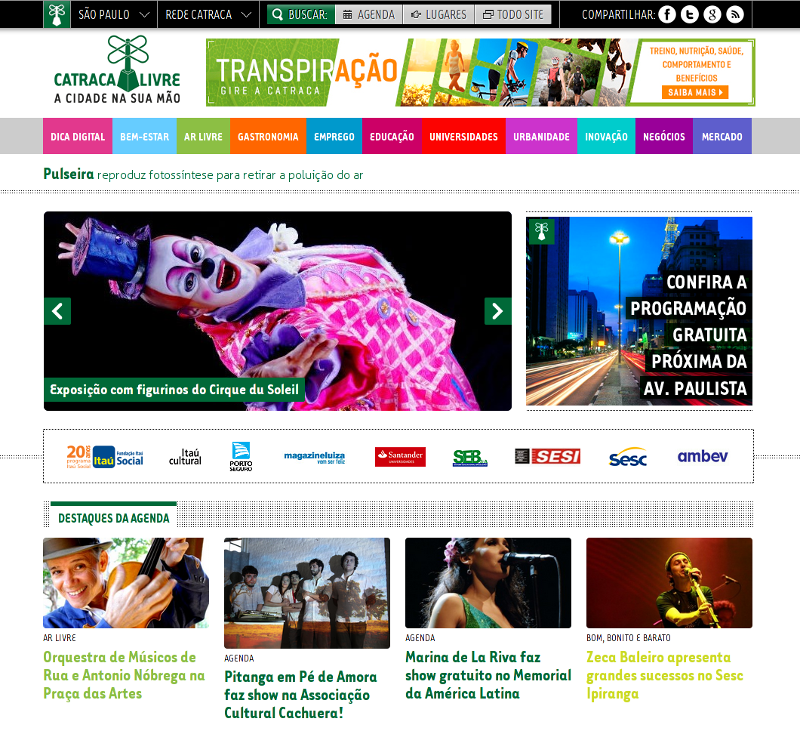
\includegraphics[height=0.8\textheight,natwidth=800,natheight=731]{./img/catracalivre.png}
  \end{center}
\end{frame}

\begin{frame}{Tratamento de conteúdo}
  \begin{itemize}
    \pause \item Funções de tratamento:
    \begin{itemize}
      \pause \item \texttt{remove\_accents()}
      \pause \item \texttt{sanitize\_title()}
      \pause \item \texttt{normalize\_whitespace()}
      \pause \item \texttt{make\_clickable()}
      \pause \item \texttt{capital\_P\_dangit()}
    \end{itemize}
  \end{itemize}
\end{frame}

\begin{frame}{Migração de mídias}
  \lstinputlisting{./code/ns-migrating-media-01.php}
\end{frame}

\begin{frame}{Migração de mídias}
  \lstinputlisting{./code/ns-migrating-media-02.php}
\end{frame}

\begin{frame}{Migração de mídias}
  \lstinputlisting{./code/ns-migrating-media-03.php}
\end{frame}

\begin{frame}{Migração de mídias: Serviço dinâmico}
  \begin{itemize}
    \item Ao invés do download com reposição, pode-se fazer o serviço dinâmico
      de mídias. Veja o arquivo \texttt{wp-includes/ms-files.php}
  \end{itemize}
\end{frame}

\begin{frame}{Migração de mídias: Serviço dinâmico}
  \lstinputlisting{./code/ns-migrating-media-dynamic-rr.txt}
\end{frame}

\begin{frame}{Migração de mídias: Serviço dinâmico}
  \lstinputlisting{./code/ns-migrating-media-dynamic.php}
\end{frame}

\subsection{URLs}

\begin{frame}{URLs}
  \begin{itemize}
    \item Para cada conteúdo migrado, sempre guardar a referência
          para o conteúdo antigo
    \pause \item Na nova estrutura, verificar os meios de acesso no conteúdo
           e redirecionar para o novo.
    \pause \item Casos:
    \begin{itemize}
      \item A partir de referências \texttt{\$\_REQUEST}
      \item A partir de regras de URL
    \end{itemize}
  \end{itemize}
\end{frame}

\begin{frame}{URLs: Referências \texttt{\$\_REQUEST}}
  \lstinputlisting{./code/url-request.php}
\end{frame}

\begin{frame}{URLs: Referências a partir de regras}
  \lstinputlisting{./code/url-rewrite-01.php}
\end{frame}

\begin{frame}{URLs: Referências a partir de regras}
  \lstinputlisting{./code/url-rewrite-02.php}
\end{frame}

\section{Considerações finais}
\subsection{Considerações finais}

\begin{frame}{Considerações finais}
  \begin{itemize}
    \pause \item Migrações devem definitivamente ser incluídas como componentes
      de projeto
    \pause \item O WordPress oferece um bom conjunto de ferramentas para se
      trazer dados para dentro de sua estrutura.
    \pause \item É cabível o desenvolvimento de plugins específicos para a
      manutenção de estruturas legadas.
    \item É mais cabível ainda utilizar estruturas externas de armazenamento
      para grandes serviços.
  \end{itemize}
\end{frame}

\end{document}
